\chapter{System Analysis}
In this chapter the challenges from the problem statement are looked into, and an overview of what will be needed to overcome these challenges, will be formulated.

%In this chapter we present the overall design of Media-Online Management(MOM). First we will present how we intend the users to use MOM. Then general concepts will be introduced which is an essential part of the system and will be mentioned several times hereafter. Thirdly the requirements of MOM will be explained in more detail. Finally the system architecture will be presented.    

\section{Designing a solution}
During the design of the system it was decided, what type of hardware that would be needed to accommodate the challenges of the problem.\\
In order to know what hardware was needed, a design of the overall solution and designation of functionality to components was needed.\\

\subsection{Identify Unique Users}
%How do we identify unique users in a subtle and child friendly way.
The first challenge in the problem statement was: ``How do we identify unique users in a subtle and child friendly way.''\\
As mentioned in the analysis there are several different ways to do this, including fingerprints and NFC tags. Common for them all is that they require some sort of scanning device to be used. For the choice of hardware see chapter \ref{chap:hardware}.\\
In order to verify that the user is actually a user on this families system this scanner must have a way to contact some sort of database or an overview of members. Which leads us to the next challenge.

\subsection{Enforce Restrictions on Media Devices}
%How do we enforce restrictions on media devices.
As mentioned in the analysis, see section \ref{section:pcHowToExtend}, it is necessary to find a way to physically restrict the usage of medias. The first thought was that the best solution would be to implement it directly into all media, but this would result in an endless amount of coding, since a code base would be needed to be implemented for each device it would run on.\\
Instead restriction is taken a bit further. Most media today run on electricity and without batteries, meaning if the power is cut to the media, it will be restricted.\\
The idea developed into a combination with the solution for the previous challenge and resulted into a ``controller''. It is a device equipped with a relay, an internet connection and a scanner.\\
Using the relay to control the power to media, using the scanner to identify users and the internet connection to look up in a sub-global\footnote{Global in the scope of each families system.} register of users, which again leads us to the next and final challenge in the problem statement. Here there is already three different devices communicating, on their own, emphasizing the idea of Internet Of Things.

\subsection{Facilitate Rules, Permissions and Chores}
%How do we facilitate concepts as rules, permission and chores without parents interaction.
Rules, permissions and chores are complicated concepts to explain which will be explained in further detail in chapter \ref{chapter:concepts}. The short version however is:\\
\textbf{Rules} is a combination of an action and a condition. Where actions could be to allow the usage of a device, give points\footnote{Points is the currency in the system that is intended to pay for media usage.} to a user or block a user. A condition could be a period of time or a repeating event such as every Monday in every week.\\
\textbf{Permissions} is a subtype of rules. Permissions is only used to tell the system the normal allowed usage of media and rules is there to overwrite these permissions in special cases, or if the user wants to customize the system.\\
\textbf{Chores} is intended as an idea to get the children to do physical activities. Parents create chores and designate a set of points that can be earned by doing this chore.\\
\\
By now there already is a lot of information in the system. There are users, rules, permissions, chores, points, timestamps and time periods, and if the system is to be extended to learn anything from the users behavior it should also include logs.\\
This is more information than should ever be put into a simple hardcoded text sheet. Meaning the system will need a database and considering that the devices has to independently be able to fetch the information they will need a good solution which would be to store the information on a server accessible by the controller.\\
Also considering the advanced concepts of rules, permissions and chores it is very likely that a graphical interface will be needed and since there already is the need for a server in our system it would make sense to make a web-site for the user to maintain edit or add these rules.\\
\\
With all these required features there is still need for specifying how they communicate and this should implement a structure that allows for changes later on. Simply because this is a prototype system and will most likely need improvements if it was to ever be commercialized or extended, which is easiest done if the system is build for it from the start.\\
\\
Next follows a section that puts the finishing touches on the system design and finally gives it a name.


\section{Media-Online Management} %name our system: temp name: Media-Online Management or MOM
The Media-Online Management (MOM) is the name of the system which is our solution on the problem statement. To give an overview of the complete system a rich picture\citep{OOAD} has been made, see the figure \ref{fig:systemoverview}. The figure shows a home environment with a TV (media), computer and an internet connection, and it shows a server connected to the system. 

There are two main use patterns. The first is a parent who manage their MOM system using the website from a PC to add, change or delete system settings. The settings will then be changed in the database as can be seen in the right side of the figure \ref{fig:systemoverview}. 

The second use pattern is pictured in the left side of the figure. It is a child user who wants to use a media which in this case is the television. But to watch television it needs power and its power source is blocked by the controller. So the child needs to scan his tag and then the controller sends a message to the server which then reply whether the television can be turned on or not. When the child is done he must scan again such that points can be withdrawn from his user profile. If the child does not have any points he cannot turn on the television nor can he turn it on if a rule or permission does not allow it. If a parent wants to watch television without being restricted in any way he can make a rule that gives him unlimited access, but he would still need to scan his tag before and after using the television. %\fixme{Vil vi lave en lille evaluering om vi synes det er fair at forældrene også skal scanne?}- nej

\begin{figure}
	\centering
		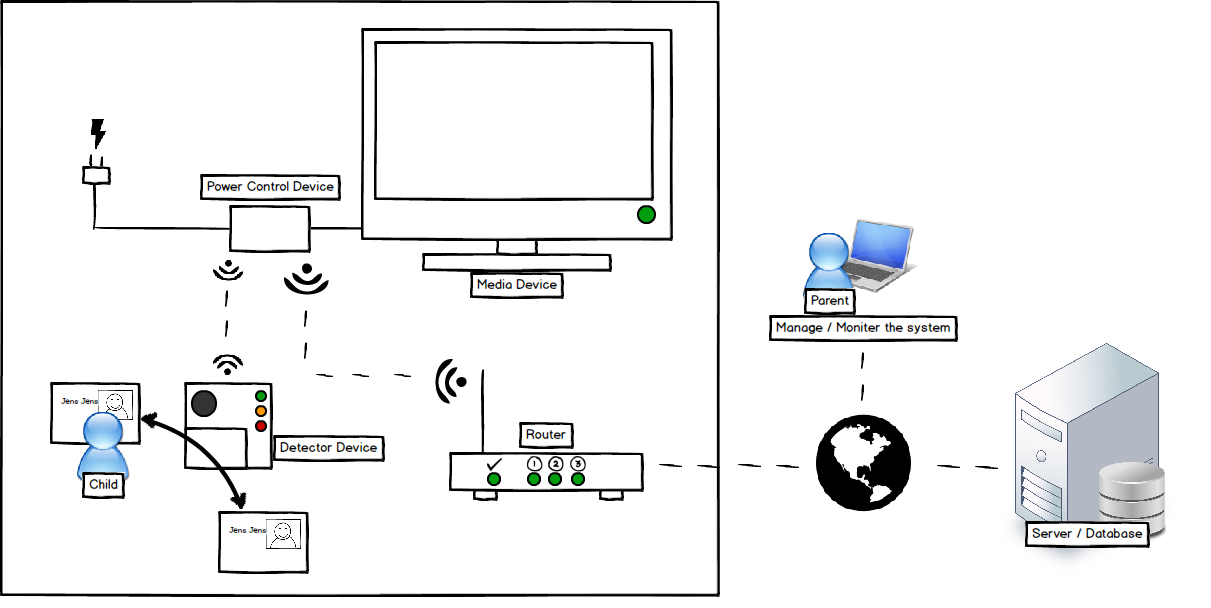
\includegraphics[width=1.50\textwidth, angle= 90]{images/systemoverview2.png}
	\caption{system overview}
	\label{fig:systemoverview}
\end{figure}

On the server there will be a database, files that generate the website, an API(a web service), and a Daemon. These elements of the system will be explained further in section \vref{chap:RequirMOM} and after that the system architecture can be presented in section \vref{sec:sysArchitecture}. However, first the hardware choices made for the system will be discussed and also the concepts of rules, permissions and chores needs to be discussed further.\\
The next chapter is about the hardware choices.